\documentclass[]{article}
\usepackage[a4paper, total={6in, 10in}]{geometry}
\usepackage[utf8]{inputenc}
\usepackage{hyperref}
\usepackage{listings}
\usepackage{graphicx}
\usepackage{caption}

\begin{document}

\begin{center}
  {\large Data Mining - ID2222}\\
  \vspace{7mm}
  {\huge Homework 5\\[1ex]}
  {\Large  Graph Spectra  }\\
  \vspace{7mm}  
  {André Silva - Jérémy Navarro\\}
  \vspace{4mm}
  {\large December 10, 2020\\}
\end{center}

\section{Overview}

In this homework, we implemented the Ja-Be-Ja algorithm by completing the provided code, as well as performed experiments using three different graphs.

Information about the structure of the project, as well as instructions on how to run it follow:

\begin{lstlisting}[language=bash]
$ unzip homework5.zip
$ ./compile.sh
$ ./run.sh -graph <path-to-graph>
$ ./plot.sh <path-to-output>
\end{lstlisting}

The project is composed by:

\begin{itemize}
    \item \texttt{src}: Source folder of the Maven project
    \item \texttt{pom.xml}: pom file of the Maven project
    \item \texttt{compile.sh}: Script to compile the project
    \item \texttt{run.sh}: Script to run the project
    \item \texttt{plot.sh}: Script to plot the results of the algorithm
\end{itemize}

\section{Task I}

\subsection{Program}

In Task 1, we completed the code in the file \texttt{Jabeja.java}, namely the functions \texttt{sampleAndSwap}, and \texttt{findPartner}.

\subsection{Results}

We then ran the program for three graphs, \texttt{3elt}, \texttt{add20}, and the Twitter graph. The results can be found in the following figures.

\begin{figure}[!h]
    \centering
    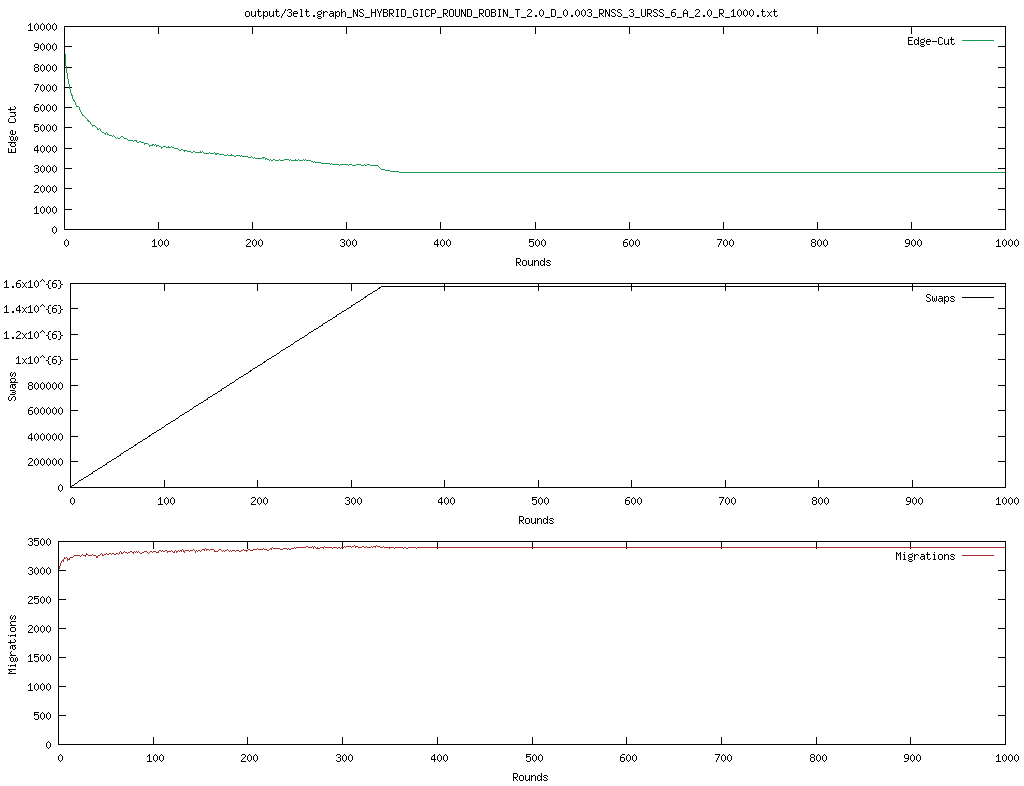
\includegraphics[width=.5\textwidth]{../3elt_noCooldDown.png}
    \caption{Result of Ja-Be-Ja for \texttt{3elt} ($T=2, \delta=0.003$)}
\end{figure}

\begin{figure}[!h]
    \centering
    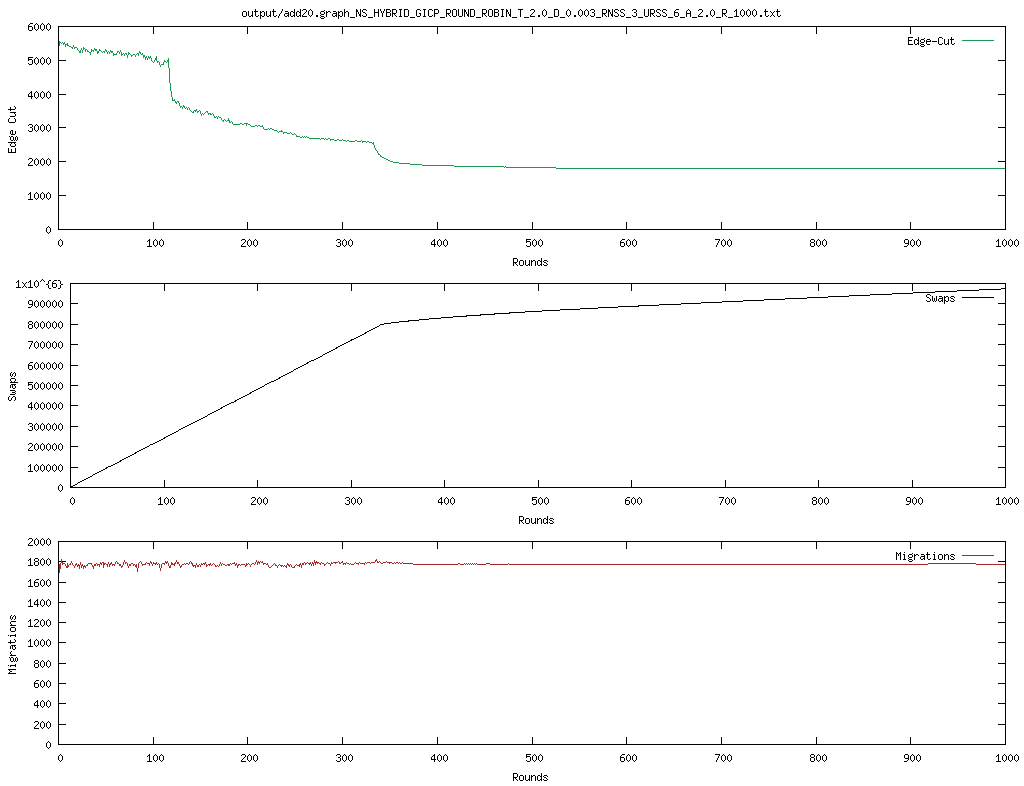
\includegraphics[width=.5\textwidth]{../add20_noCooldDown.png}
    \caption{Result of Ja-Be-Ja for \texttt{add20} ($T=2, \delta=0.003$)}
\end{figure}

\begin{figure}[!h]
    \centering
    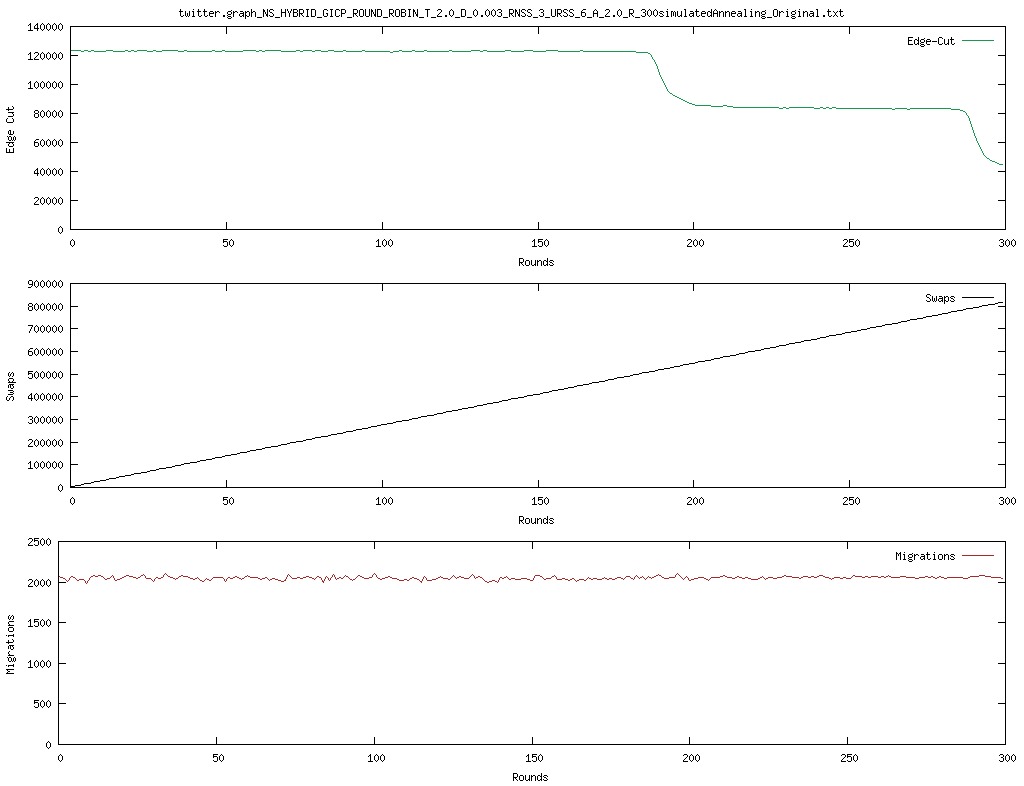
\includegraphics[width=.5\textwidth]{../task2/twitter.graph_NS_HYBRID_GICP_ROUND_ROBIN_T_2.0_D_0.003_RNSS_3_URSS_6_A_2.0_R_300simulatedAnnealing_Original.txt.png}
    \caption{Result of Ja-Be-Ja for the Twitter graph ($T=2, \delta=0.003$)}
\end{figure}

\pagebreak

\section{Task II}

\subsection{Program}

In Task 2, we implemented the simulated annealing mechanism, in the function \texttt{saCoolDown}.

\subsection{Results}

We then ran, again, the program for the same three graphs, experimenting with different values of $\alpha$, $\delta$, and the effect of restarting the simulated annealing mechanism.

\begin{table}[!h]
\begin{tabular}{|l|l|}
\hline
                                                                                   & Edge-Cut \\ \hline
Result of Ja-Be-Ja for \texttt{3elt} ($T=2, \delta=0.01$)                          & 2982     \\ \hline
Result of Ja-Be-Ja for \texttt{3elt} ($T=2, \delta=0.003$)                         & 2788     \\ \hline
Result of Ja-Be-Ja (w/ simulated annealing) for \texttt{3elt} ($T=1, \alpha=0.3$)  & 3199     \\ \hline
Result of Ja-Be-Ja (w/ simulated annealing) for \texttt{3elt} ($T=1, \alpha=0.5$)  & 2970     \\ \hline
Result of Ja-Be-Ja (w/ restart) for \texttt{3elt} ($T=1, \alpha=0.5$)              & 2646     \\ \hline
Result of Ja-Be-Ja (w/ simulated annealing) for \texttt{add20} ($T=1, \alpha=0.3$) & 1938     \\ \hline
Result of Ja-Be-Ja (w/ simulated annealing) for \texttt{add20} ($T=1, \alpha=0.5$) & 1953     \\ \hline
Result of Ja-Be-Ja (w/ restart) for \texttt{add20} ($T=1, \alpha=0.5$)            & 1898     \\ \hline
Result of Ja-Be-Ja (w/ simulated annealing) for Twitter graph ($T=1, \alpha=0.3$)  & 40952    \\ \hline
Result of Ja-Be-Ja (w/ simulated annealing) for Twitter graph ($T=1, \alpha=0.5$)  & 42079    \\ \hline
Result of Ja-Be-Ja (w/ restart) for Twitter graph ($T=1, \alpha=0.5$)              & 41013    \\ \hline
\end{tabular}
\end{table}

\begin{figure}[!h]
    \centering
    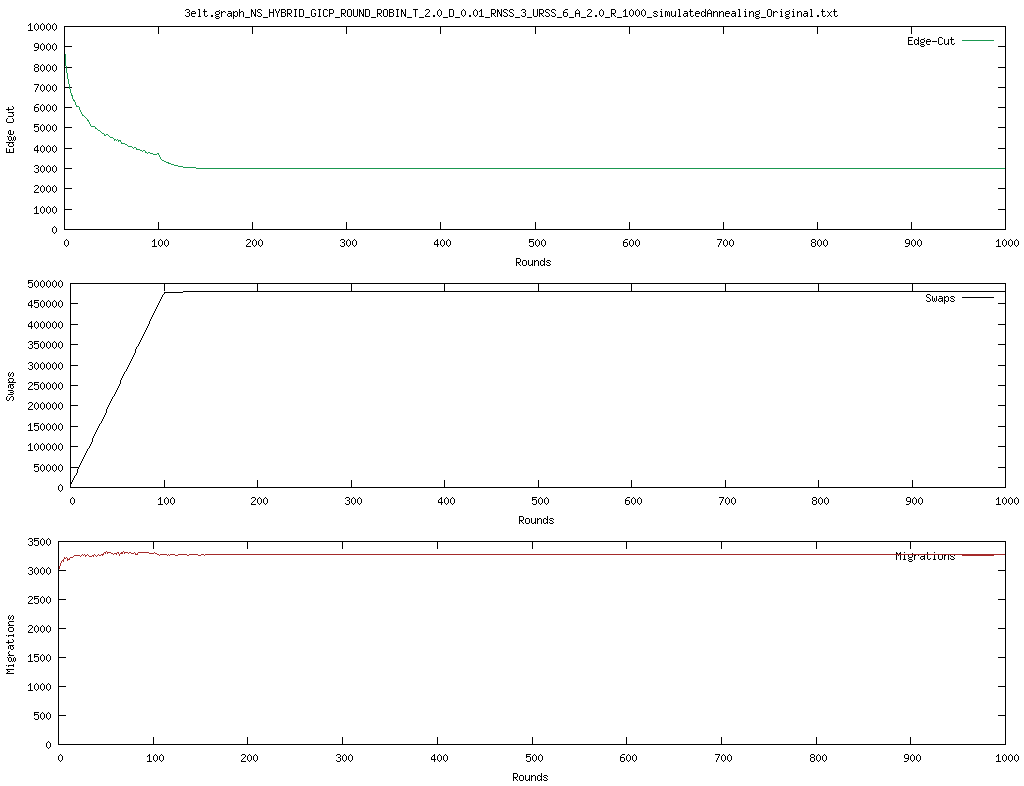
\includegraphics[width=.5\textwidth]{../task2/3elt.graph_NS_HYBRID_GICP_ROUND_ROBIN_T_2.0_D_0.01_RNSS_3_URSS_6_A_2.0_R_1000_simulatedAnnealing_Original.txt.png}
    \caption{Result of Ja-Be-Ja for \texttt{3elt} ($T=2, \delta=0.01$)}
\end{figure}

\begin{figure}[!h]
    \centering
    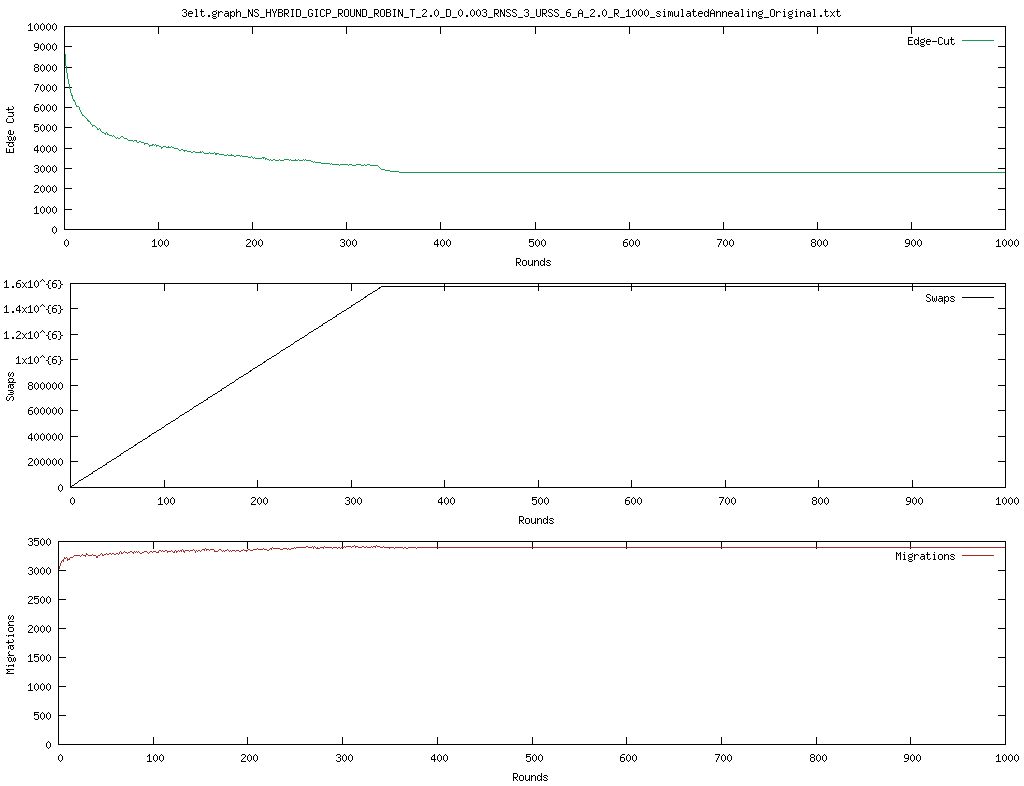
\includegraphics[width=.5\textwidth]{../task2/3elt.graph_NS_HYBRID_GICP_ROUND_ROBIN_T_2.0_D_0.003_RNSS_3_URSS_6_A_2.0_R_1000_simulatedAnnealing_Original.txt.png}
    \caption{Result of Ja-Be-Ja for \texttt{3elt} ($T=2, \delta=0.003$)}
\end{figure}

\begin{figure}[!h]
    \centering
    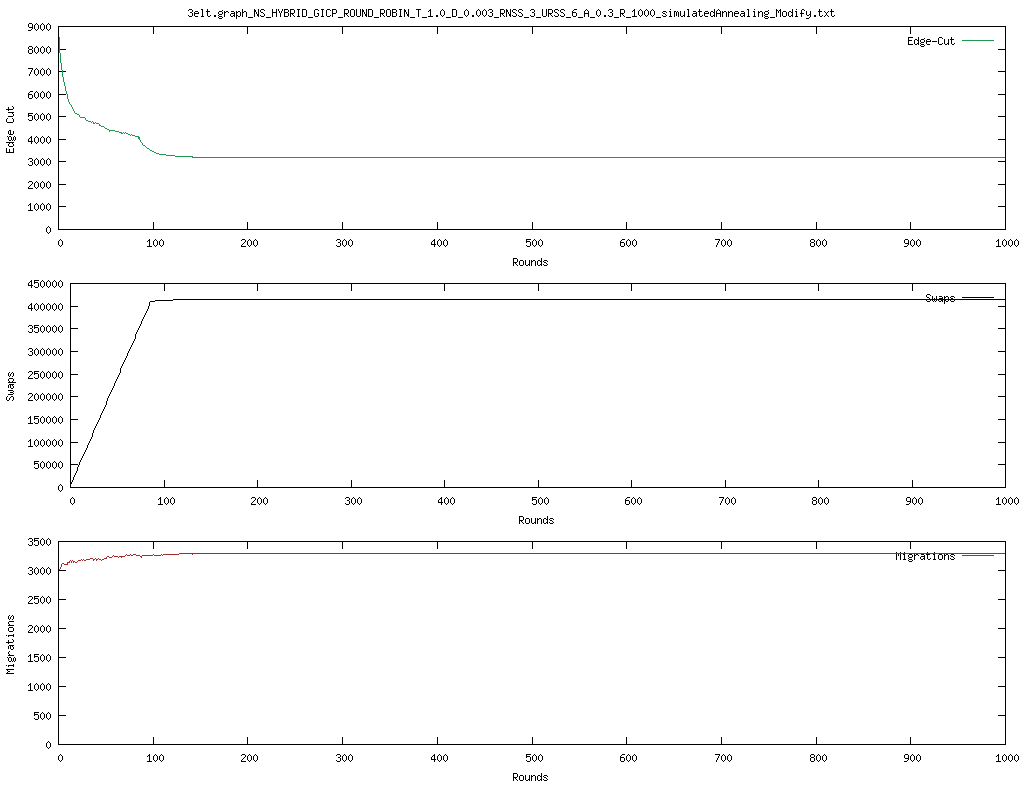
\includegraphics[width=.5\textwidth]{../task2/3elt.graph_NS_HYBRID_GICP_ROUND_ROBIN_T_1.0_D_0.003_RNSS_3_URSS_6_A_0.3_R_1000_simulatedAnnealing_Modify.txt.png}
    \caption{Result of Ja-Be-Ja (w/ simulated annealing) for \texttt{3elt} ($T=1, \alpha=0.3$)}
\end{figure}

\begin{figure}[!h]
    \centering
    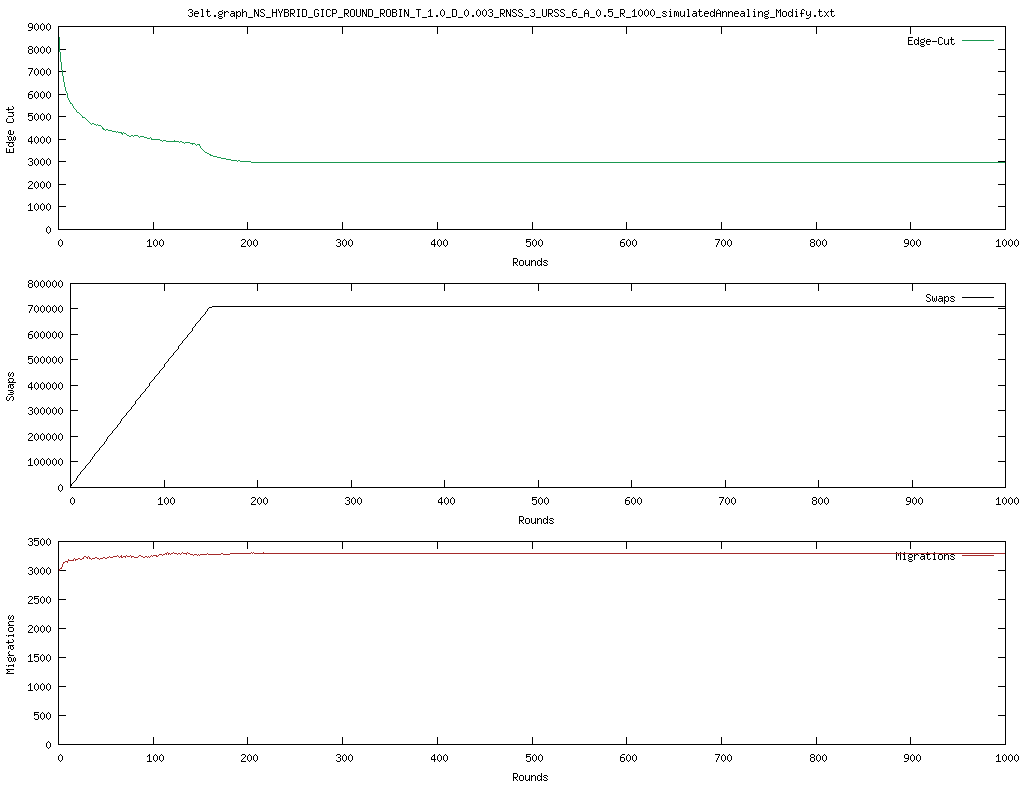
\includegraphics[width=.5\textwidth]{../task2/3elt.graph_NS_HYBRID_GICP_ROUND_ROBIN_T_1.0_D_0.003_RNSS_3_URSS_6_A_0.5_R_1000_simulatedAnnealing_Modify.txt.png}
    \caption{Result of Ja-Be-Ja (w/ simulated annealing) for \texttt{3elt} ($T=1, \alpha=0.5$)}
\end{figure}


\begin{figure}[!h]
    \centering
    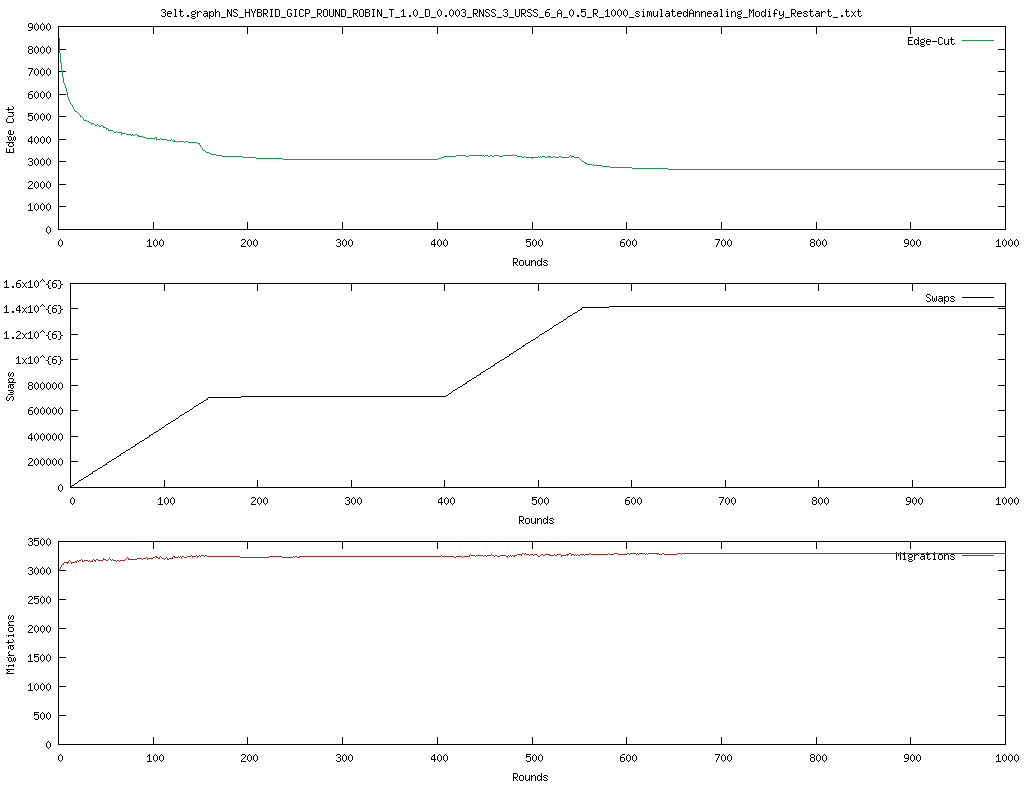
\includegraphics[width=.5\textwidth]{../task2/3elt.graph_NS_HYBRID_GICP_ROUND_ROBIN_T_1.0_D_0.003_RNSS_3_URSS_6_A_0.5_R_1000_simulatedAnnealing_Modify_Restart_.txt.png}
    \caption{Result of Ja-Be-Ja (w/ restart) for \texttt{3elt} ($T=2, \alpha=0.5$)}
\end{figure}

\pagebreak

\begin{figure}[!h]
    \centering
    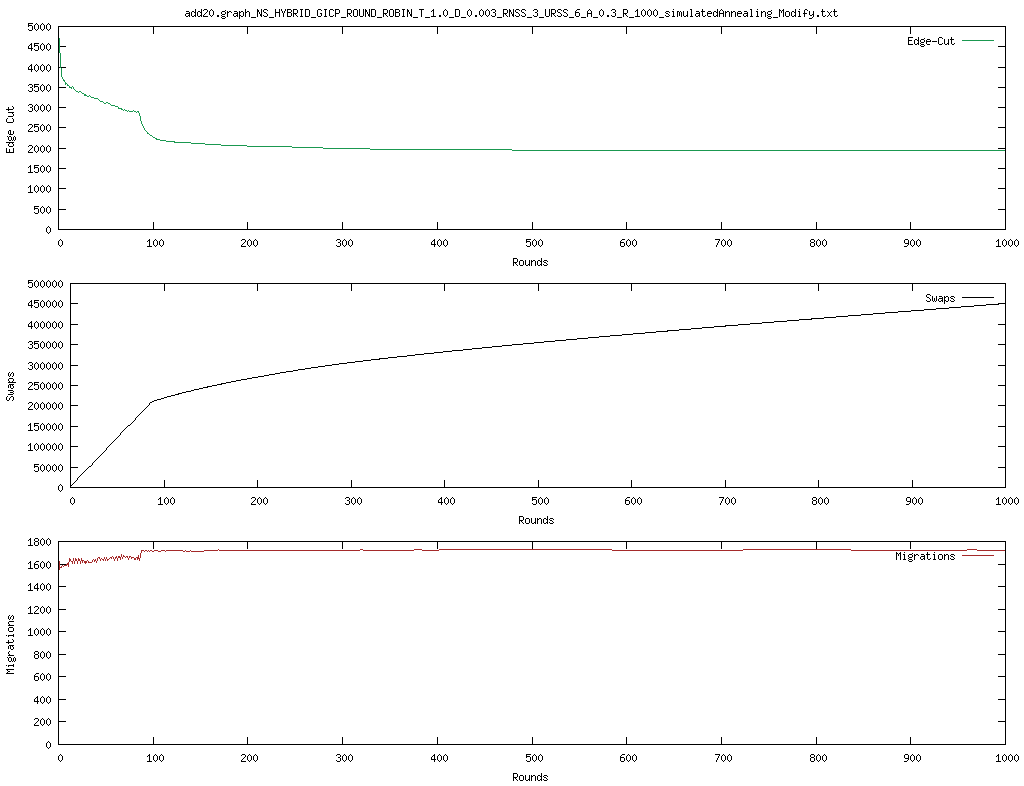
\includegraphics[width=.5\textwidth]{../task2/add20.graph_NS_HYBRID_GICP_ROUND_ROBIN_T_1.0_D_0.003_RNSS_3_URSS_6_A_0.3_R_1000_simulatedAnnealing_Modify.txt.png}
    \caption{Result of Ja-Be-Ja (w/ simulated annealing) for \texttt{add20} ($T=1, \alpha=0.3$)}
\end{figure}

\begin{figure}[!h]
    \centering
    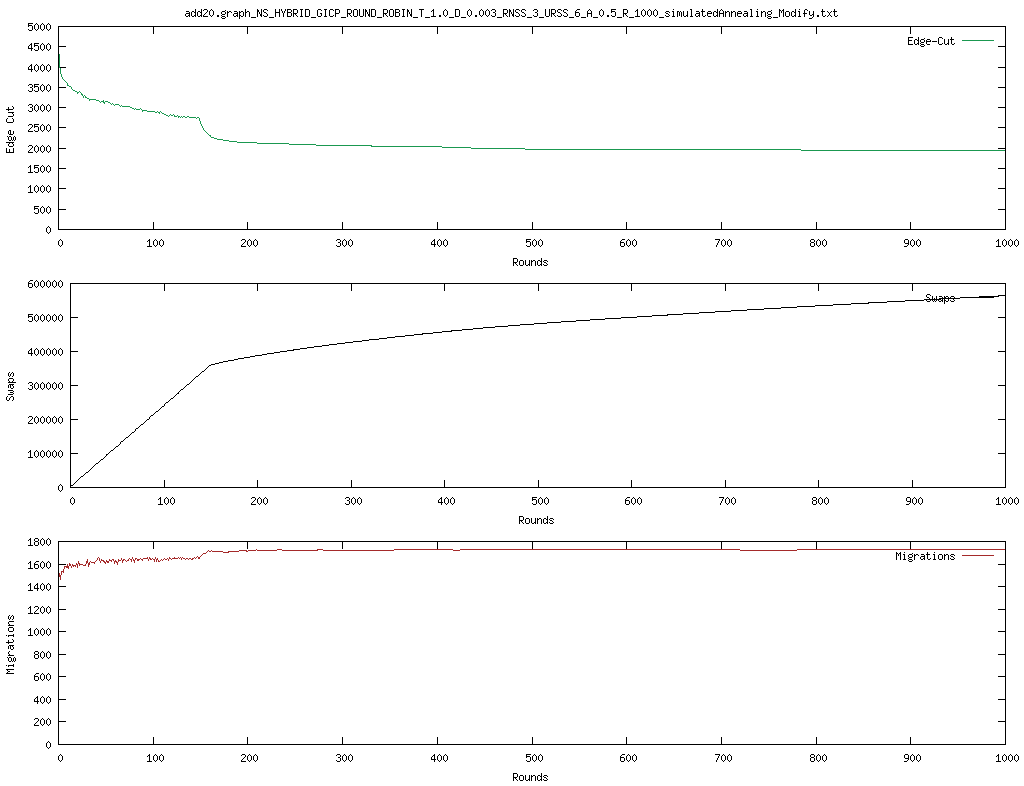
\includegraphics[width=.5\textwidth]{../task2/add20.graph_NS_HYBRID_GICP_ROUND_ROBIN_T_1.0_D_0.003_RNSS_3_URSS_6_A_0.5_R_1000_simulatedAnnealing_Modify.txt.png}
    \caption{Result of Ja-Be-Ja (w/ simulated annealing) for \texttt{add20} ($T=1, \alpha=0.5$)}
\end{figure}


\begin{figure}[!h]
    \centering
    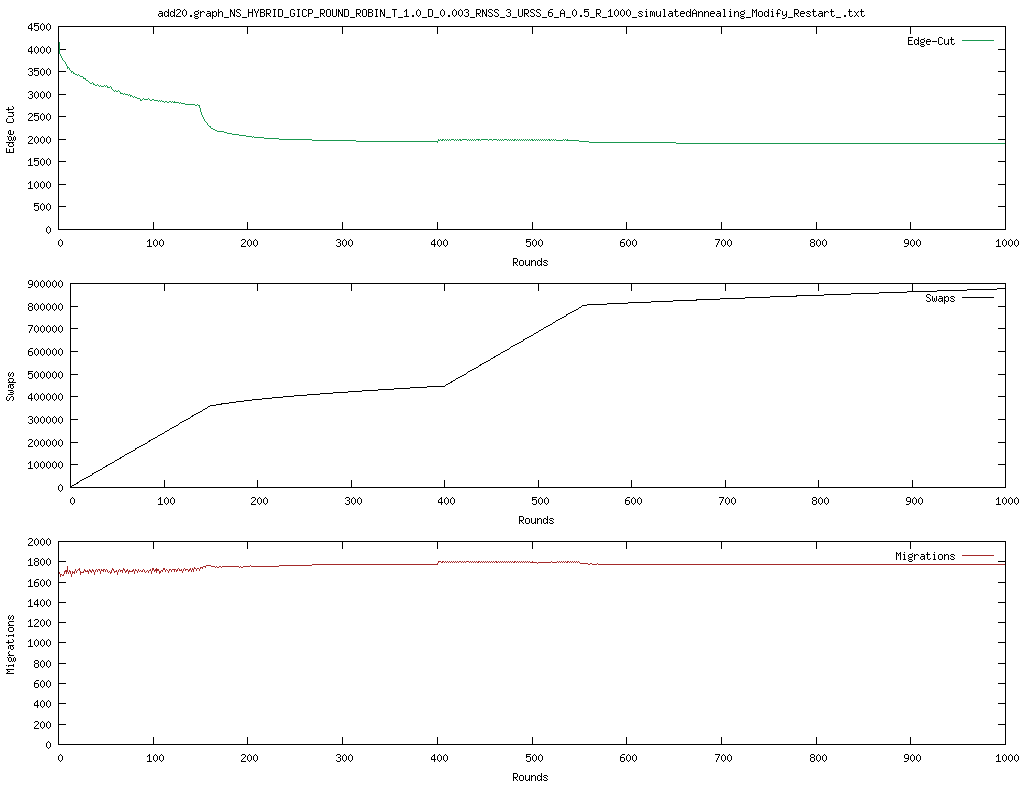
\includegraphics[width=.5\textwidth]{../task2/add20.graph_NS_HYBRID_GICP_ROUND_ROBIN_T_1.0_D_0.003_RNSS_3_URSS_6_A_0.5_R_1000_simulatedAnnealing_Modify_Restart_.txt.png}
    \caption{Result of Ja-Be-Ja (w/ restart) for \texttt{add20} ($T=1, \alpha=0.5$)}
\end{figure}

\pagebreak

\begin{figure}[!h]
    \centering
    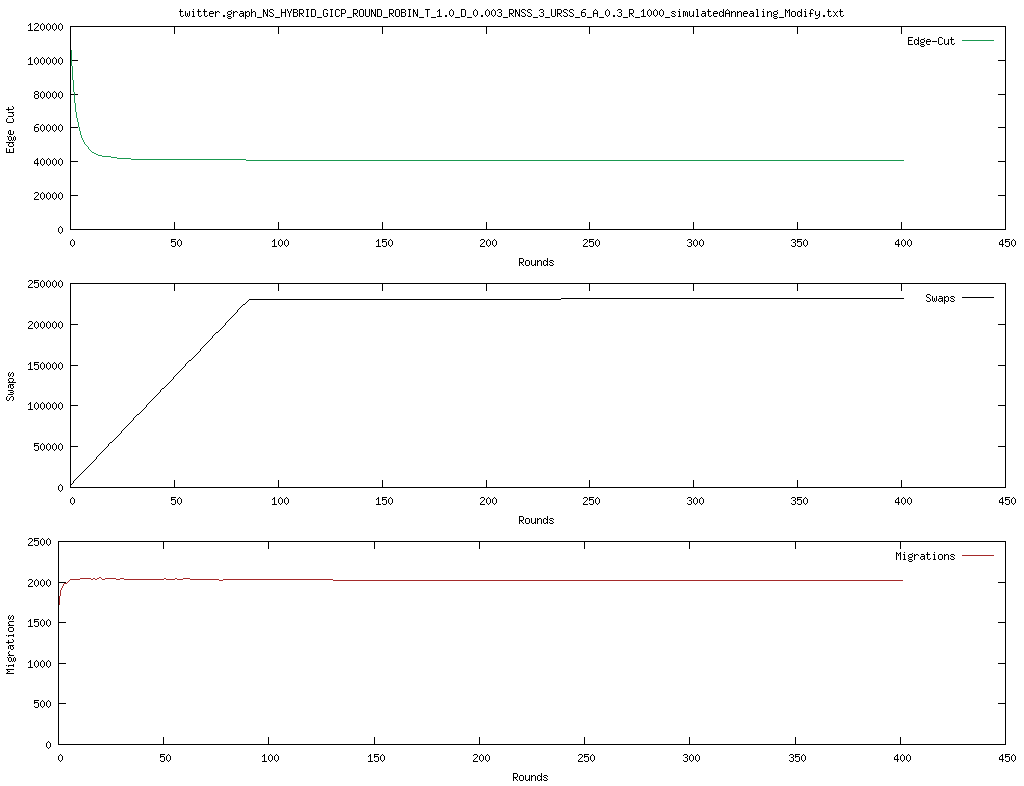
\includegraphics[width=.5\textwidth]{../task2/twitter.graph_NS_HYBRID_GICP_ROUND_ROBIN_T_1.0_D_0.003_RNSS_3_URSS_6_A_0.3_R_1000_simulatedAnnealing_Modify.txt.png}
    \caption{Result of Ja-Be-Ja (w/ simulated annealing) for Twitter graph ($T=1, \alpha=0.3$)}
\end{figure}

\begin{figure}[!h]
    \centering
    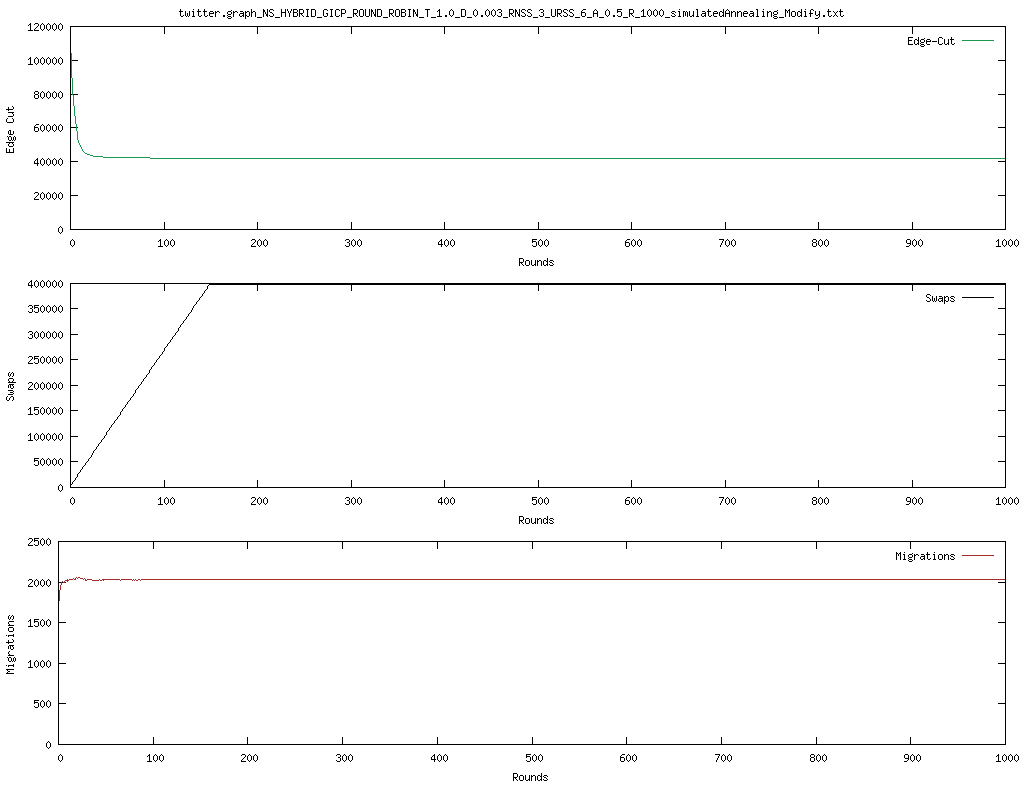
\includegraphics[width=.5\textwidth]{../task2/twitter.graph_NS_HYBRID_GICP_ROUND_ROBIN_T_1.0_D_0.003_RNSS_3_URSS_6_A_0.5_R_1000_simulatedAnnealing_Modify.txt.png}
    \caption{Result of Ja-Be-Ja (w/ simulated annealing) for Twitter graph ($T=1, \alpha=0.5$)}
\end{figure}


\begin{figure}[!h]
    \centering
    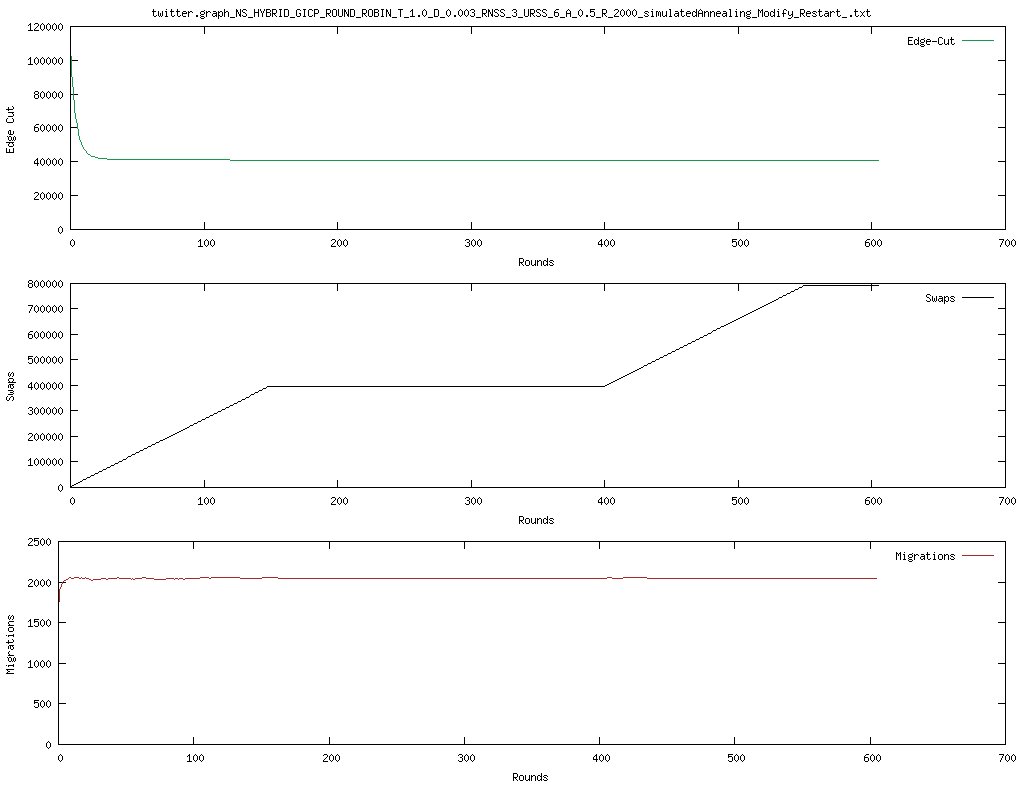
\includegraphics[width=.5\textwidth]{../task2/twitter.graph_NS_HYBRID_GICP_ROUND_ROBIN_T_1.0_D_0.003_RNSS_3_URSS_6_A_0.5_R_2000_simulatedAnnealing_Modify_Restart_.txt.png}
    \caption{Result of Ja-Be-Ja (w/ restart) for Twitter graph ($T=1, \alpha=0.5$)}
\end{figure}

\end{document}
